\chapter{Mathematical basics}
\section{Diffie-Hellman key exchange}
\begin{center}
\begin{figure}[!htb]
    \centering
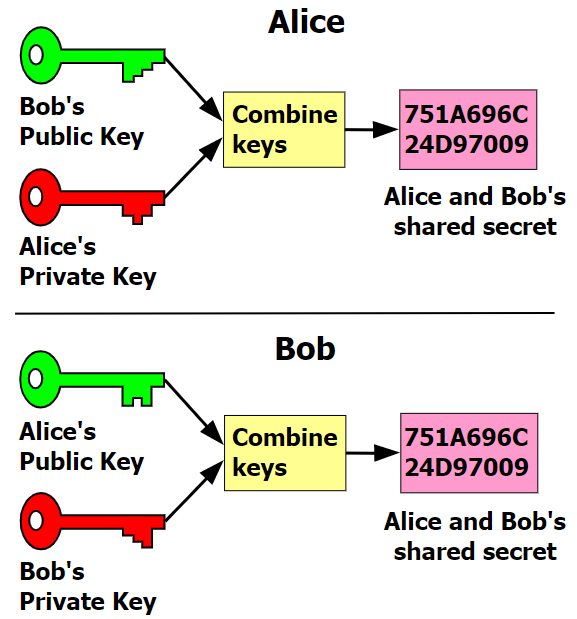
\includegraphics[width=6cm,height=8cm,keepaspectratio]{DHKeyExchange}
    \caption{Diffie Hellman key exchange}
    \label{fig:DHKeyExchange}
\end{figure}
\end{center}
\newline
The Diffie Hellman Key Exchange is a key agreement protocol. It allows two communication partners to agree on a common secret key via a public non-secure channel. This agreed secret key can then be used for a symmetric cryptosystem.
There are now different variants of the Diffie Hellman Key Exchange procedure, which are also used in various corners of the Internet.\cite{Diffie-Hellman_key_exchange}
\subsection{Mathematical basics}
In the following chapters, the mathematical basics of the asymmetric crypto methods based on the discrete logarithm are explained. The Diffie Hellman Key Exchange is composed of various mathematical aspects. The essential aspects that are necessary for the design and security analysis of the Diffie Hellman Key Exchange are explained in more detail in the following chapters.
\subsubsection{One-way function}
A Diffie Hellman Key Exchange uses certain mathematical basics, one of these basics is the one-way function(s). 
A one-way function is a mathematical function that is "easy" to calculate in terms of complexity theory, but very "difficult" to reverse. 
\begin{displaymath} \text{A mathematical one-way function }  f : X \to Y  \text{ must satisfy the following properties:}\end{displaymath}
    \begin{displaymath}
    \text{The calculation of }  y = f(x)  \text{ is "easy".}
    \end{displaymath}
This means that an algorithm exists that can calculate the value in polynomial time.
\newline
\begin{displaymath}
\text{The calculation of } f^-1(y) = x \text{is "hard".}
\end{displaymath}
This means that there is no "fast" algorithm for this problem that could solve it in polynomial time.\cite{Robshaw2011}
\subsubsection{Discrete exponential function and discrete logarithm}
The discrete exponential function \(b^x\mod m\) return the remainder when dividing \(b^x\) by m. 
And the inverse of the discrete exponential function is called discrete logarithm.
\newline
The big advantage of discrete exponential functions is that they can be calculated efficiently even with large exponents. So even functions with a number of more than hundred bits can be calculated within a second on the PC if implemented cleverly. For this to happen efficiently, both Euler's theorem
\newline 
(For all \(a, n \in \mathbb{N}\) with \(ggT(a,n) = 1\)
applies \(a^\varphi^(^n^) \equiv 1 (\mod n)\))
\newline 
as well as the Square & Multiply method are used.
\newline
But for the inverse, i.e. the discrete logarithm \(f(x) = b^x\modm\), no efficient and fast algorithm is known yet. Even with the greatest hardware effort and the best known algorithms, one only achieves calculation times that exceed the lifetime of our universe. Therefore, it can be assumed that the discrete exponential function is a one-way function according to today's knowledge. \cite{Diffie-Hellman_key_exchange}
\newpage
\subsubsection{Group theory}
Group theory deals with the algebraic structures of groups in mathematical space. 
Accordingly, a group consists of a set of things (numbers, symbols, objects, motions) and a calculus (a linkage \(*\)) that specifies how to deal with the set. This calculation rule is bound to certain rules, the so-called group axioms:
\begin{itemize}
    \item The combination of two elements of the set results in an element of the same set. (Completeness of the set)
    \item For the combination of the elements the bracketing is not of importance, i.e., it is valid \((a * b) * c = a * (b * c)\) for all \(a,b,c\). (associative law)
    \item There is an element \(\varepsilon\) in the set, which does nothing with respect to the conjunction, i.e. a \(*\)-neutral element:\(a * \varepsilon = \varepsilon * a = a\) for all \(a\)
    \item For each element \(a\) there is a reverse element with respect to the link, i.e. an \(*\text{-inverse}\) element \(a^*\). This element has the property of yielding the neutral element when it is linked with \(a\): \(a^* * a = a * a^* = \varepsilon\).
\end{itemize}
A group is therefore defined as follows: It is a pair \((G, *)\). Here \(G\) is a set and \(*\) is the linkage to \(G\). 
The following figure can be described accordingly:  \cite{Diffie-Hellman_key_exchange}
\begin{eqnarray*}
*: G \times G \to G (a, b) \mapsto a * b
\end{eqnarray*}
\subsubsection{Prime residual class group}
In arithmetic, the integers relatively prime to n from the set \(\{0,1,....,n-1\}\) of \(n\) non-negative integers form a group under multiplication of modulo \(n\).
This group is called the multiplicative group of integers modulo \(n\).
\newline
This type of group plays a significant role in cryptography because they are finite abelian groups with respect to multiplication.
An important property of the prime residue class is that for every prime residue class \(a + n\mathbb{Z}\) there exists a prime residue class \(b + n\mathbb{Z}\) such that holds:
\begin{eqnarray*}
ab \equiv 1 \pmod n
\end{eqnarray*}
The prime residue class \(b + n\mathbb{Z}\) is therefore the inverse element of \(a + n\mathbb{Z}\) with respect to the multiplication in the prime residue class group \(\mathbb{Z}^*_n\).\cite{Multiplicative_group_of_integers_modulo_n}
\newpage
\subsubsection{Primitive root modulo n}
Certain elements of prime residue class groups are called primitive roots in scale theory. The primitive root has a primitive property, through this property it is possible to represent each element of the primitive residue class group by means of one of its powers.
For example, the number 3 is a primitive root modulo 7, since holds:\cite{Primitive_root_modulo_n}
\begin{eqnarray*}
3^1\equiv3  \pmod 7 \\
3^2\equiv2  \pmod 7 \\
3^3\equiv6  \pmod 7 \\
3^4\equiv4  \pmod 7 \\
3^5\equiv5  \pmod 7 \\
3^6\equiv1  \pmod 7 \\
\end{eqnarray*}
\section{Elliptic Curves}
Elliptic curves are special algebraic curves on which addition is geometrically defined. They play an important role in cryptography to construct secure encryption methods. This due to the various properties of elliptic curves. For example, the discrete logarithm problem is much harder to compute on an elliptic curve than on finite solids.  
For the representation of elliptic curves, so-called affine planes with a point at infinity are used. 
However, elliptic curves can also be defined in arbitrary bodies, but only elliptic curves over finite bodies are used in cryptography.
\newline
\newline
An elliptic curve is defined as follows according to Willems.
\newline
Let \(\mathbb{K}\) be a body of characteristic not equal to 2 and 3. 
\newline
A polynomial equation of the form \(\text{E: }y^2 = x^3 + ax + b\) with \(a, b \in \mathbb{K}\) with discriminant \(\Delta = 4a^3 + 27b^2 \neq 0\) is called an elliptic curve.
\newline
The condition \(\Delta \neq 0\) ensures that the polynomial \(x^3 + ax + b\) has three pairwise different zeros.\cite{ellipticCurves}
\newpage
\subsection{Elliptic Curve Diffie-Hellman (ECDH)}
The elliptic curve Diffie Hellman (ECDH) differs from the general Diffie Hellman in that it is based on the discrete logarithm problem of the elliptic curve (ECDLP) as opposed to the discrete logarithm problem (DLP) of the general Diffie Hellmann. The Elliptic Key Diffie Hellmann is an anonymous key agreement protocol that allows 2 parties to share a secret over a insecure channel. Each party has a public-private key pair, of which only the public key is used for the exchange. The private key remains with the party and is needed to create the shared secret.
\newline
The ECDH works as follows. A and B agree on the elliptic curve group \(\mathbb{E}\) of order \(n\) and \(a\) primitive element \(\mathbb{P}\) in \(\mathbb{E}\), which then also has the order \(n\). \(\mathbb{E} \text{, } n \text{ and } \mathbb{P}\) are assumed to be known to the adversary. The ECDLP, which the ECDH is based on, is defined as the computation of the integer \(k\) given \(\mathbb{P} \text{ and } \mathbb{Q}\) such that \(\mathbb{Q} = [k]\mathbb{P}\). The ECDH
let A and B compute a shared secret key S, using the property of the ECDLP as described below. A selects an integer \(a\) in the range [2, n-1], computes
\(\mathbb{Q} = [a]\mathbb{P}\) and sends \(\mathbb{Q}\) to B. B on the other hand selects an integer \(b\) in the range [2, n-1], computes \(\mathbb{R} = [b]\mathbb{P}\) and sends \(\mathbb{R}\) to A. A and B receives \(\mathbb{R} \text{ and } \mathbb{Q}\) respectively, and computes the shared secret key 
S; \(S = [a]\mathbb{R} = [b]\mathbb{Q} = [a][b]\mathbb{P} = [a ∗ b \mod{n})]\mathbb{P}\). Both A and B get the same value for S, and the shared key is established.\cite{ECDH}
\newline
\begin{center}
\begin{figure}[!htb]
    \centering
    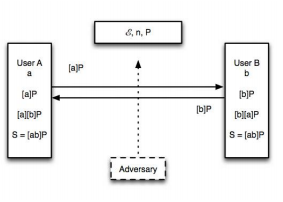
\includegraphics[width=9cm,height=11cm,keepaspectratio]{ecdh}
    \caption{Elliptic curve Diffie Hellman}
    \label{fig:ecdh}
\end{figure}
\end{center}
\newpage